The Minimal Effort model is a \textit{mean field model}, needful to capture interesting behaviors in object-oriented programming. In addition, it is useful to introduce a \textit{microscopic model}, the Sharing tree model, which gives you a method to create inheritance structures and so which allows the construction of Monte Carlo trees, for data comparisons.

%%%%%%%%%%%%%%%%%%%%%%%%%%%%%%%%%%%%%%%%%%%%%%%%%%%%%%%%%%%%%%%%%%%%%%%%%%%%%
\section{Random objects}
Our starting point is a set of $\Enne$ classes which represents the computer science solution of a given problem. 

Consider each class composed by a set of different symbols randomly extracted from an alphabet. While the alphabet represents the whole writable code, each symbol represents a unit of code, as in the mean field model.

Each class is composed by a set of $\kappa$ symbols, and there are $\Esse$ symbols equally likely in the alphabet. This is a first approximation that allows you to find analytic results, but in principle not all units of code are equally important and used and not all classes have the same size.

The metric to measure the size of a code is an open question. The most popular method is \textit{counting source line of code}, subgrouped in physical lines (the whole code) and logical lines (the number of statements), but it is not necessarily an honest method. The same task can be performed by two different programs of different sizes and with different statements and you cannot know in advance whether the best program is the largest or the smallest.

A reasonable starting point is to consider classes of the same size, represented by $\kappa$, and a simplified alphabet where the $\Esse$ symbols are equally likely.

\begin{figure}[p]%
\center
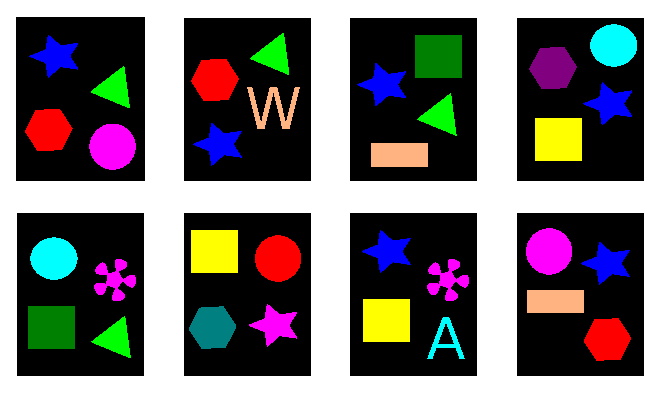
\includegraphics[width=7cm,draft=false]{images/sequenze.eps}
\caption{\label{Sequenza} \footnotesize\textbf{Example of initial sets} - In this $\Enne=8$ classes, only $\enne=6$ contain the most common symbol, the blue star.}
\vspace{2cm}
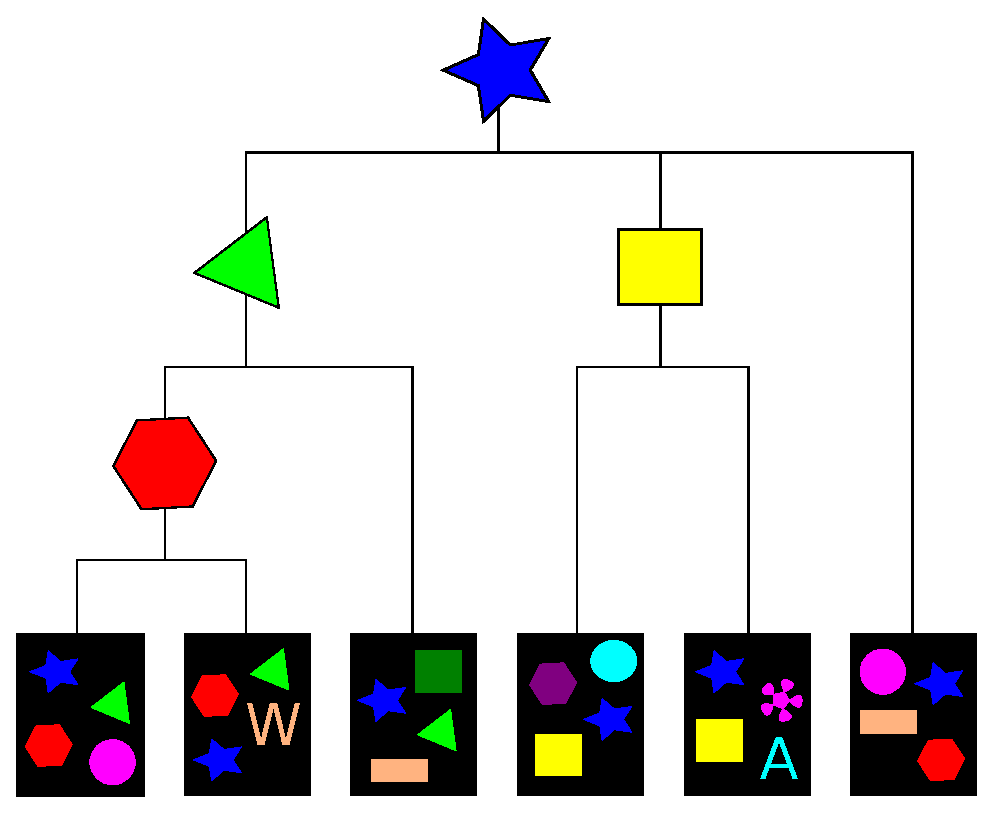
\includegraphics[width=\textwidth,draft=false]{images/sharingtree.eps}
\caption{\label{Albero} \footnotesize\textbf{Sharing Tree} - The most common symbol rule allows the creation of a tree. The $\enne$ classes represent the leaves, while each symbol chosen as the most common represents an internal node.}
\end{figure}

\section{Building the structure}
Once selected the $\Enne$ classes, rules are necessary to decide the structure of the tree. And so, how can we group classes in order to build a tree structure?

First, select the symbol that appears more often in the $\Enne$ classes. Keep classes with this symbol and delete the others. This symbol will be our root, and so the part of the code that all nodes of our tree hold in common. With the excluded classes one can in principle constructs other trees, but for now let just delete them.

The next step is the selection of the symbol that appears more often in the remaining $\enne$ classes. This symbol represents the second node of the tree, connected to the root only, for now.  

If $j$ classes contain this second symbol, we need to find the most common symbol in the $\enne-j$ remaining classes. The symbol is the third node, connected to the root. This process is iterated for all remaining classes until clustering is finished. The most common symbol groups all the classes in sets composed by different elements and with different number of element in each group. Furthermore, sets of one class are allowed: they are reminders of groupment, appearing once or even more times if the reminder is composed of more classes that hold nothing in common and for which the most common symbol rule does not work.

Each symbol used to group classes represents a node connected to the root, but it represents also a set of classes that have been grouped with such symbol.

When a group contains a single class, it means that its process is finished, but for each group with two or more classes the process can be iterated. The number of iterations necessary to finally arrive to all sets of one class only is $\Elle$, and it is exactly the depth of the tree. In fact, each step increases tree depth by one while it decreases the available symbols and the elements of each class by one (for this reason, $\kappa$ cannot be too small!).

Therefore, the process is finished when no group contains more than one class or when classes have no more symbols to be shared.

%%%%%%%%%%%%%%%%%%%%%%%%%%%%%%%%%%%%%%%%%%%%%%%%%%%%%%%%%%%%%%%%%%%%%%%%%%%%%%%%%%%%%%
\section{Most common symbol}
The key concept underlying the mechanism that grows trees from classes is the \textit{most common symbol rule}. Selecting the symbol that appears more often, we are applying an optimization principle: we are not interested in a random groupage, but in the best groupage in a certain defined sense.

It is not trivial to describe how the most common symbol is distributed, but with some calculations we can obtain lots of interesting results that substantially solve the model.

Then, to be quantitatively and to find analytical solutions we must find the answer to a probabilistic question: what is the occurrence of the most common symbol in $\Enne$ sets of $\kappa$ draws from an alphabet of $\Esse$ symbols without replacement?

The answer to this question is central for the model. Each groupage done to build the tree, follows the very same most common symbol rule. The analytic solution that we are looking for can be applied iteratively (with opportune parameters) in order to describe the distribution of the number of classes in each set and at each step. In a certain number of steps, sets become singletons and the process is over.

\subsection{Find a symbol in a sequence}
Unlike the choice made in the Minimal Effort model, Sharing Tree model symbols cannot be repeated in a sequence. Such refinement simplifies the following calculation but it also approaches the model to real classes in which code repetition does not have a well defined sense.

Thus, the probability to find a selected symbol in a sequence is given by the hypergeometric distribution
\[ p = \frac{\binom{\Esse-1}{\kappa-1}}{\binom{\Esse}{\kappa}}= \frac{\kappa!(\Esse -1)!}{\Esse!(\kappa -1)!} \]

\subsection{How many classes for each symbol?}
In how many classes does such symbol appear? The answer is given by the Binomial distribution of $\Enne$ trials in which the symbol can appear or not with probability $p$.

The Binomial distribution then describes the occurrence $w$ of each symbol in the $\Enne$ sequences. We can compute the probability that $w$ classes contain a selected symbol with
\[ Pr(w) = \binom{\Enne}{w} \, p^{w} \, (1-p)^{\Enne-w} \]

\subsection{What about the most common symbol?}
In the Sharing tree model, optimization is carried by the choice of the most common symbol, and not any one of them.

Let's say that each symbol $s \in \Esse$ appears in $w_s$ classes. The set $\{w_s\}_{s=1}^{\Esse}$ contains $\Esse$ random variables independent and identically distributed, and the most common symbol is the one that appears $\omega$ times
\[ \omega = \max \left\{ w_1, \dots, w_{\Esse} \right\} \]

In order to find the distribution of the occurrence of the most common symbol, it is necessary to do some calculations. Therefore, consider the cumulative distribution function of $\omega$
\[ F_{\omega} (y)= Pr(\omega \leq y) \]
Since $\omega$ is the maximal occurrence and the $w_s$ are independent, it holds that
\begin{align*}
Pr(\omega \leq y) &= Pr(w_1 \leq y, w_2 \leq y, \dots, w_{\Esse} \leq y) \\
&= Pr(w_1 \leq y) Pr(w_2 \leq y) \dots Pr(w_{\Esse} \leq y)
\end{align*}
and since all $w_s$ have the same cumulative mass function, we can write
\[ F_{\omega} (y) = F_{w}^{\Esse} (y) \]

The probability distribution of $\omega$ can now be obtained as the probability that $\omega \leq y$ minus the probability that $\omega \leq y-1$, and so
\begin{align*}
Pr (y = \omega) &= Pr (\omega \leq y) - Pr (\omega \leq y-1) \\
&= F_w^{\Esse} (y) - F_w^{\Esse} (y-1)
\end{align*}

\subsection{Probability distribution of most common symbol}
The occurrence of the most common symbol now is straightforward. Remembering that $w_s$ are binomial random variables, the occurrence $\omega$ of the most common symbol is therefore distributed as 
\[\Psi (\omega) = \left( \sum_{i=0}^{ \omega} \text{Bin}(\Enne, i) \right)^{\Esse}- \left( \sum_{i=0}^{\omega -1} \text{Bin}(\Enne, i) \right)^{\Esse}\]

Making explicit the formula of the Binomial distribution, we have finally obtained the distribution of the occurrence of the most common symbol
\[\Psi (\omega) = \left( \sum_{i=0}^{ \omega} \binom{\Enne}{i} p^i (1-p)^{\Enne -i} \right) ^{\Esse}- \left( \sum_{i=0}^{\omega -1} \binom{\Enne}{i} p^i (1-p)^{\Enne -i}\right) ^{\Esse} \]

Examples of this distribution for different parameters are shown in figures \ref{Tpsi1} and \ref{Tpsi2}.

\begin{figure}[p]%
\center
\includegraphics[width=\textwidth,draft=false]{grafici/campana1.eps}
\caption{\label{Tpsi1} \footnotesize\textbf{The function $\Psi (\omega)$ } - This figure represent the probability distribution of the occurrence of the most common symbol in $5000$ sequences of $100$ extracted symbols (without repetitions) from an alphabet of $2000$ symbols.}
\vspace{1cm}
\includegraphics[width=\textwidth,draft=false]{grafici/campana2.eps}
\caption{\label{Tpsi2} \footnotesize\textbf{$\Psi (\omega)$ for different parameters} - Some examples of the probability distribution of the occurrence of the most common symbol for different parameters.}
\end{figure}

\subsection{Mean occurrence of the most common symbol}
To make the calculations less demanding, often it is useful to deal with the mean instead of the whole distribution. We can obtain $\langle \omega \rangle$ expanding
\[ \langle \omega \rangle = \sum_{\omega = 1}^{\Enne} \omega \Psi(\omega) \]

To obtain the final simplified formula, some calculations are needed and in order to ease the notation, we can define $a_{\omega}$ as
\[a_{\omega} = \left( \sum_{i=0}^{ \omega} \binom{\Enne}{i} p^i (1-p)^{\Enne -i} \right) ^{\Esse} \]
and then rewrite $\Psi (\omega)$ as
\[\Psi (\omega) = a_{ \omega} - a_{ \omega-1} \]

Inserting the formula in the mean occurrence of the most common symbol, we have
\[\langle \omega \rangle = \sum_{\omega = 1}^{\Enne} \omega \left(a_{ \omega} - a_{ \omega-1}\right) \]
which is a telescopic series, that allows an important simplification 
\begin{align*}
\langle \omega \rangle &= 1\left(a_{1} - a_{0}\right) + 2\left(a_{2} - a_{1}\right)+ \dots + \Enne\left(a_{\Enne} - a_{\Enne-1}\right) \\
&= \Enne a_{\Enne} - a_{0} - a_{1} - \dots - a_{\Enne-1}
\end{align*}
Furthermore, considering that $a_{\Enne}$ is the sum over all possible cases of a probability, it is equal to $1$. Then we finally obtain
\[ \langle \omega \rangle = \Enne - \sum_{j=0}^{\Enne -1} a_j \]

Thus, the mean of the distribution of the occurrence of the most common symbol is explicitly
\[ \langle \omega \rangle =  \Enne - \sum_{j=0}^{\Enne -1} \left( \sum_{k=0}^{j} \binom{N}{k} p^k (1-p)^{\Enne -k} \right)^\Esse \]

With this formula, we can study directly how parameters change the mean of the number of leaves (but not of total nodes) of simulated trees, as shown in figure \ref{TwN}. Considering that, at each step, the groupage of classes in the process is made with the same rule, the formula for $\langle \omega \rangle$ can be applied iteratively to find the mean of the number of classes in each set and for each step of the recursive groupage.

\begin{figure}[p]%
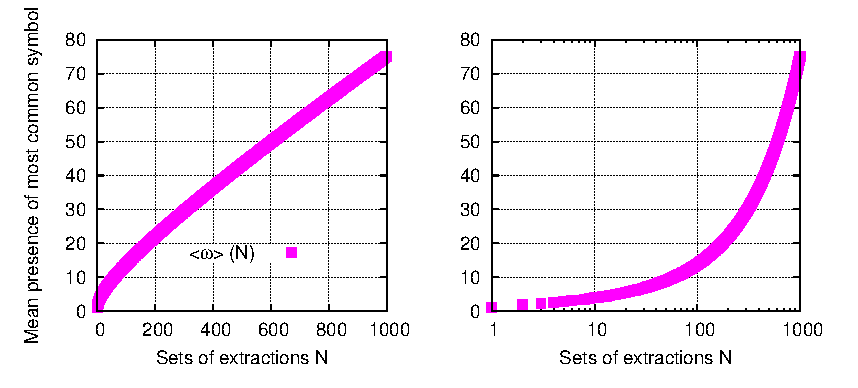
\includegraphics[width=\textwidth,draft=false]{grafici/meanN.eps}
\includegraphics[width=\textwidth,draft=false]{grafici/meank.eps}
\includegraphics[width=\textwidth,draft=false]{grafici/meanS.eps}
\caption{\label{TwN} \footnotesize\textbf{The mean occurrence $\langle\omega\rangle$ } - In the first figure, $\Esse$ and $\kappa$ are fixed at $\Esse = 2000$ and $\kappa = 100$ while and $\langle\omega\rangle$ is plotted as a function of $\Enne$. In the second figure $\Enne =500$ and $\Esse=2000$. In the third one, $\Enne=500$ and $\kappa=50$.}
\end{figure}

\section{Sharing process}
The recipe to build the tree can be seen also as the set of rules defining a process.

At each step, the recipe suggest to look for the symbol that appear more often and to group classes inspired by \textit{most common symbol rule}.

Following the iteration, the number of nodes are $ x_0 = \Enne, x_1, \dots , x_{\Elle} = 1$. Every time we divide classes in \textit{with} or \textit{without} the most common symbol, the process generate $\eta$ subprocesses, with $\eta$ the minimum number of subgroups necessary to cover all available classes.

Consider only the main process, which starts from $\Enne$ classes and which divides them into 2 subgroups, iteratively until the $x_{\Elle}$ is reached. All other subprocesses behave in the same manner with the opportune initial condition.

The mean number of elements of a group at each step $t$ is given by
\[ f(x_t, t) = x_t - \sum_{j=0}^{x_t-1} \left( \sum_{i=0}^{j} \binom{x_t}{i} \Pi_t^i \left( 1 - \Pi_t \right)^{x_t-i} \right)^{\Esse-t} \]
where $\Pi_t$ is obtained with the hypergeometric distribution and considering that if a symbol has been used as \textit{the most common} then it cannot be reused, and so at each step $\Esse \to \Esse -1$ and $\kappa \to \kappa -1$.
\[ \Pi_t = \frac{\binom{\Esse-1-t}{k-1-t}}{\binom{\Esse-t}{\kappa-t}} = \frac{\Gamma(\Esse-t)\Gamma(\kappa-t+1)}{\Gamma(\kappa-t)\Gamma(\Esse-t+1)}\]

The process for the mean number of elements can so be defined as
\[ x_{t+1} = f(x_{t},t) \]
where $x_0=x(0)$ and is equal to $\Enne$ for the main process.
%The initial condition is defined by the number of available classes, $x_0 = \Enne$.
%
\comment{
%\section{Alphabet and drawings}
%We need $\kappa\enne$ extraction. We can choose $\kappa$ and $\Esse$ with $\kappa < \Esse$ and then $\enne$ satisfying 
%\[ Z(\Esse) = \sum_{i=0}^{\Esse-1} \frac{\Esse}{\Esse-i} = \Esse\left (1+\frac{1}{2}+\frac{1}{3}+\dots+\frac{1}{\Esse} \right ) \]
%so that extractions are more then the mean minimum number necessary to span all the alphabet.
%If $\kappa\enne > Z(\Esse)$, all the alphabet is spanned.
%\begin{figure}[ht]%
%\center
%\includegraphics[width=9cm,draft=false]{grafici/wdiesse.eps}
%\caption{\label{Tesse} \footnotesize\textbf{The function Z(S)} }
%\end{figure}
}
%%%%%%%%%%%%%%%%%%%%%%%%%%%%%%%%%%%%%%%%%%%%%%%%%%%%%%%%%%%%%%%%%%%%%%%%%%%%%%%%%%%%%%%%%%%%%%%%%%
\section{Monte Carlo simulations}
What kinds of trees arise from Sharing Tree Monte Carlo simulations? To give an answer to this question, I have written a C++ code and I have integrated it with the data analysis library. The program is well optimized and fast and each tree is obtained in few seconds or less for all parameters that have been chosen.

In this section the simulations and the study of the behavior of trees are presented for different parameters.

\begin{figure}[p]%
\includegraphics[width=\textwidth,draft=false]{grafici/Tnodes.eps}
\caption{\label{Tnodi} \footnotesize\textbf{Initial nodes and number of leaves} - The mean number of leaves is a linear function of the initial number of nodes. The fit leads to $y=0.06x + 18$ when $k=100$ and $S=2000$. The function $\Psi (\omega)$ explains perfectly the leaves distribution.}
\vspace{1cm}
\includegraphics[width=\textwidth,draft=false]{grafici/Ttotnodes.eps}
\caption{\label{Ttotnodes} \footnotesize\textbf{Total nodes for different initial nodes} - While the distribution of total nodes is spread, its mean is linear in the number of initial nodes, with $y=0.2x + 58.7$ when $k=100$ and $S=2000$.}
\end{figure}

%------------------------
\subsection{Initial nodes and leaves}
This model does not allow you to fix the number of leaves of a tree, but only the number of initial nodes, among which leaves will be selected. Once fixed the $\Enne$ initial nodes, the tree will be built with a number of leaves whose dependence from this parameter has been obtained in the previous section and showed in figure \ref{TwN}.

In the range in which simulations were made, the mean number of leaves $\enne$ is substantially linear respect to the number of initial nodes $\Enne$, as shown on the left hand side of figure \ref{Tnodi}. This means that we can easily decide the mean number of leaves of simulated trees multiplying the number of initial nodes by the factor obtained from the linear fit.

The simulated distribution perfectly matches the analytic solution for the distribution of the most common symbol, as shown on the right hand side of figure \ref{Tnodi}, where the function $\Psi (\omega)$ exactly overlap the distribution of the number of leaves once fixed $\Enne$, $\Esse$ and $\kappa$.

%------------------------
\subsection{Total number of nodes}
The number of nodes in a tree consists in the number of leaves increased by the number of symbols used by the process. Due to the random nature of the number of leaves, the total number of nodes in a tree is usually a spread distribution.

Anyway, the mean is a linear function of the initial nodes and this allows to easily control the mean number of nodes of trees.

%------------------------
\subsection{Trees depth}
The depth $\Elle$ represents the number of steps in which all sets of classes, or sequences, have become singletons. In simulations, it has a sharp distribution, as showed on the right hand side of figure \ref{Tdepth}.

It is not surprising, since the number of classes in sets is strongly suppressed by each step of the process, with a small variance that decreases as a function of the number of classes, as deducible from figures \ref{TwN} and \ref{Tpsi2}.

The mean depth is a logarithmic function of initial nodes, as shown on the left hand side of figure \ref{Tdepth}. Since initial nodes are a linear function of total nodes, the logarithmic behavior of the depth is exactly the same result obtained from the Minimal Effort model. This is an optimal behavior for comparisons with data.

\begin{figure}[p]%
\includegraphics[width=\textwidth,draft=false]{grafici/Tdepth.eps}
\caption{\label{Tdepth} \footnotesize\textbf{Depth for different initial nodes} - Depth of trees has a sharp distribution, and the mean is a logarithmic function of the initial nodes, as $y=1.1\log(x) + 6.6$.}
\vspace{1cm}
\includegraphics[width=\textwidth,draft=false]{grafici/Toutdeg.eps}
\caption{\label{Toutdeg} \footnotesize\textbf{Outdegrees for different initial nodes} - The mean of outdegrees approaches $1$ for increasing number of initial nodes, while outdegrees distribution show a bizarre sharp peak for high outdegree.}
\end{figure}

%------------------------
\subsection{Outdegrees}
The outdegrees distribution shows an interesting behavior. While its mean approaches the value of $1$ for increasing number of initial nodes, as shown on the left hand side of figure \ref{Toutdeg}, the distribution of outdegrees is concentrated in low outdegree, but with a sharp peak of occurrence for high outdegree, as shown on the right hand side of \ref{Toutdeg}.

This means that some nodes share their code with lots of nodes, or in model terminology, that few symbols are used to group lots of nodes that have little more in common.

The gap in the distribution of outdegrees between the \textit{normal nodes} and \textit{special nodes} gradually becomes more and more pronounced while the number of initial node becomes higher, as detailed shown in figure \ref{TEoutdeg}.

This behavior can be investigated more closely studying the outdegree as a function of some variable, and this will be done in next section.

\begin{figure}[p]%
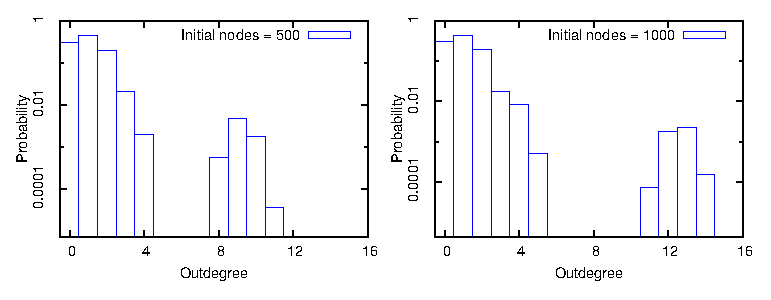
\includegraphics[width=\textwidth,draft=false]{grafici/TEXoutdeg1.eps}
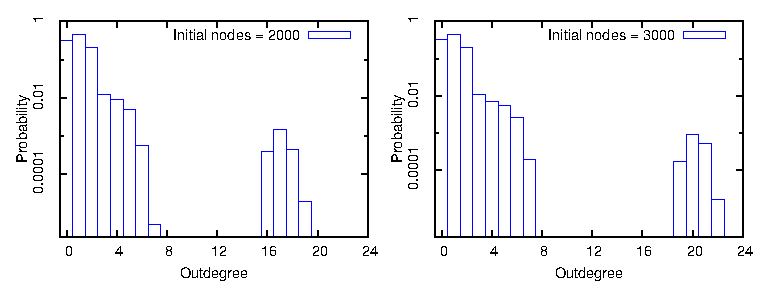
\includegraphics[width=\textwidth,draft=false]{grafici/TEXoutdeg2.eps}
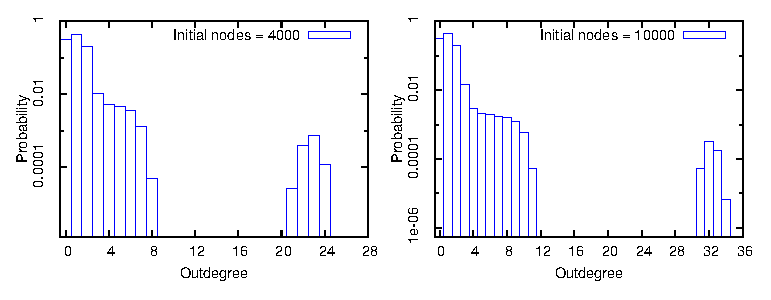
\includegraphics[width=\textwidth,draft=false]{grafici/TEXoutdeg3.eps}
\caption{\label{TEoutdeg} \footnotesize\textbf{Outdegrees distribution for different initial nodes} - The gap in the distribution of outdegrees becomes more and more pronounced while the number of initial node becomes higher.}
\end{figure}

%------------------------
\subsection{Outdegree mean per level}
A useful description of tree topology is the outdegree mean as a function of levels. In the Minimal Effort model we have seen how this function couples with the depth and that it shows a growth close to the root, strong or weak depending on the depth of the tree.

The microscopic rules of the Sharing Tree model lead to a very similar behavior. As shown on the top of figure \ref{Koutlev}, simulations build trees with an outdegree mean which grows with levels and which has a strong growth near the root.

Parameters govern the position and the height of peaks. In the bottom of figure \ref{Koutlev}, $\kappa$ and $\Esse$ are fixed, while $\Enne$ varies. The increase of the number of initial nodes moves the peak, and the depth, to higher levels and to higher outdegrees mean. More nodes need to been grouped, but they does not have many symbols in common.

On the top of figure \ref{KKoutlev}, the varying parameter is $\kappa$. When $\kappa$ is small, the depth is small since few symbols are available for groupage. When $\kappa$ grows, the height of the peaks does not change since it is coupled only with the number of leaves, and so with the number of initial nodes.

On the bottom of figure \ref{KKoutlev}, $\Esse$ is varying. The depth change with $\Esse$ and peaks move slowly while the number of possible symbols in $\Esse$ increases.

The behavior of outdegree mean as a function of level can be changed through the probability of each symbol in the alphabet. In this chapter, all symbols in alphabet are equally likely, but if some symbols would have more probability to be chosen in the extractions respect the others, we may expect a decline of peaks for higher depths. If there are few symbols with which we can initially group classes, then the outdegree mean of high levels will be lower, at least for one level. This argument will be useful in data analysis.

\begin{figure}[p]%
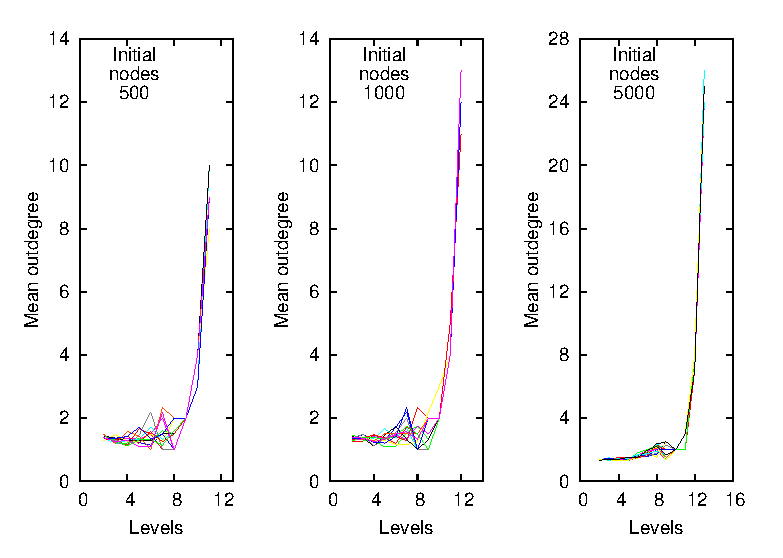
\includegraphics[width=\textwidth,draft=false]{grafici/ToutVSlev.eps}
\includegraphics[width=\textwidth,draft=false]{grafici/VoutVSlev3.eps}
\caption{\label{Koutlev} \footnotesize\textbf{Outdegree mean per level} - On the top, the figure shows some examples of outdegree mean as a function of levels for different initial nodes and with fixed depth. The figure on the bottom shows how the parameter $\Enne$ can change the simulated trees.}
\end{figure}

\begin{figure}[p]%
\includegraphics[width=\textwidth,draft=false]{grafici/VoutVSlev.eps}
\includegraphics[width=\textwidth,draft=false]{grafici/VoutVSlev2.eps}
\caption{\label{KKoutlev} \footnotesize\textbf{Outdegree mean per level} - Figures shows how parameters move the main quantities in simulated trees, as the depth and outdegrees distribution.}
\end{figure}

